\documentclass[tikz, border=2mm]{standalone}
\usepackage{tikz,pgfplots, caption}
\usetikzlibrary{decorations.pathreplacing,calligraphy}
\usetikzlibrary{fadings}

\begin{document}
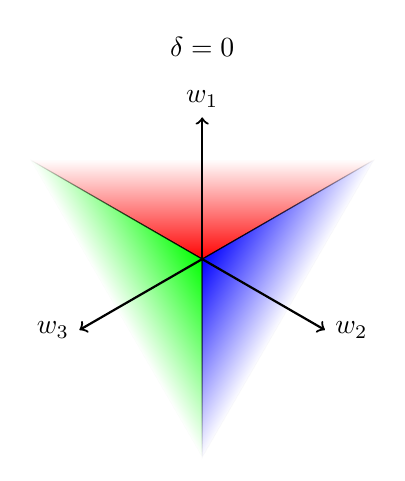
\begin{tikzpicture}[scale=1.8]
    \node at (0,1.5) {$\delta = 0$};
    \node at (0,-1.3) { };

    \filldraw[fill=red, path fading=north] (0,0) -- (30:1.4) -- (150:1.4) -- (0,0);
    \begin{scope}[transform canvas={rotate=120}]
        \filldraw[fill=green, path fading=north] (0,0) -- (30:1.4) -- (150:1.4) -- (0,0);
    \end{scope}
    \begin{scope}[transform canvas={rotate=240}]
        \filldraw[fill=blue, path fading=north] (0,0) -- (30:1.4) -- (150:1.4) -- (0,0);
    \end{scope}

    \draw[->, thick] (0,0) -- (90:1) node [above] { $w_{1}$};
    \draw[->, thick] (0,0) -- (330:1) node [right] { $w_{2}$};
    \draw[->, thick] (0,0) -- (210:1) node [left] { $w_{3}$};
\end{tikzpicture}
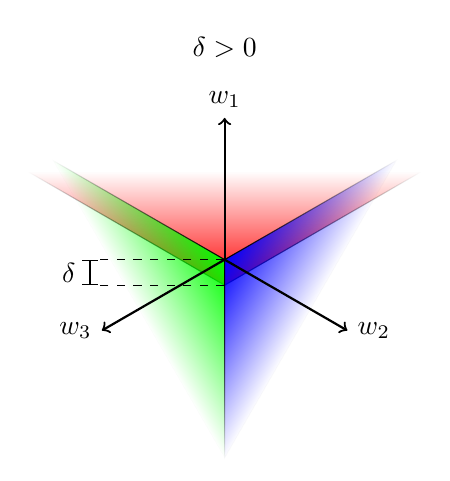
\begin{tikzpicture}[scale=1.8]
    \node at (0,1.5) { $\delta > 0$};
    \node at (0,-1.3) { };

    \filldraw[fill=red, path fading=north, shift={(0,-0.18)}] (0,0) -- (30:1.6) -- (150:1.6) -- (0,0);
    \begin{scope}[transform canvas={rotate=120}]
        \filldraw[fill=green, path fading=north] (0,0) -- (30:1.4) -- (150:1.4) -- (0,0);
    \end{scope}
    \begin{scope}[transform canvas={rotate=240}]
        \filldraw[fill=blue, path fading=north] (0,0) -- (30:1.4) -- (150:1.4) -- (0,0);
    \end{scope}
    \draw[->, thick] (0,0) -- (90:1) node [above] { $w_{1}$};
    \draw[->, thick] (0,0) -- (330:1) node [right] { $w_{2}$};
    \draw[->, thick] (0,0) -- (210:1) node [left] { $w_{3}$};

    \draw[dashed] (0,0) -- (-0.9,0);
    \draw[dashed] (0,-0.18) -- (-0.9,-0.18);

    \draw[|-|] (-0.95,0) -- (-0.95,-0.18);
    \node at (-1.1,-0.09) {$\delta$};

\end{tikzpicture}

\end{document}
